%
% latex-sample.tex
%
% This LaTeX source file provides a template for a typical research paper.
%

%
% Use the standard article template.
%
\documentclass{article}
\usepackage[affil-it]{authblk}
\usepackage{multirow}
% The geometry package allows for easy page formatting.
\usepackage{geometry}
\geometry{letterpaper}

% Load up special logo commands.
\usepackage{doc}

% Package for formatting URLs.
\usepackage{url}

% Packages and definitions for graphics files.
\usepackage{graphicx}
\usepackage{epstopdf}
\DeclareGraphicsRule{.tif}{png}{.png}{`convert #1 `dirname #1`/`basename #1 .tif`.png}

%
% Set the title, author, and date.
%
\title{Interim Report of "Hadoop YARN Cloud Configuration Tool"}

\author{Group 9: Shiqian Xu, Jiang Gu, Pengyu Li, Liang Dong}
\affil{Course: Data Intensive Computing}
\date{2015-10-19}

%
% The document proper.
%
\begin{document}

% Add the title section.
\maketitle
\newpage
% Add an abstract.
\section{Abstract}
Data analytics is becoming increasingly prominent in a variety of application areas ranging from extracting business intelligence to processing data from scientific studies. Hadoop Cluster works well to these data-intensive analytics jobs, given its ability to scale-out and leverage several machines to parallely process data. In this project, we will deploy Hadoop Cluster on AWS cloud platform using Apache Ambari and docker images, and monitor runtime information of the Hadoop eco-system by running different data sets and create a model based these runtime information. Based on our model, we can make a decision when to scale out Hadoop Cluster by adding or deleting data nodes. Then we present a scale solution and strategy of how to scale out Hadoop Cluster and compare the Hadoop Cluster performance of before scale and after scale using different data sets.
	
\section{Introduction}
This paper gives a description on how to deploy Hadoop YARN cluster using Apache Ambari, monitor the cluster and later on use the monitoring data to scale the cluster by adding or deleting data nodes based on status of the instance or job type. \textbf{Figure 1} gives an overview on the whole system looks like.

\begin{figure}[h!]
 \centering
  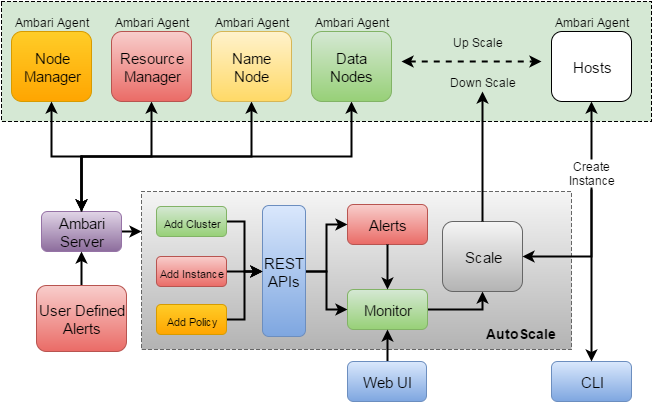
\includegraphics[width=0.7\textwidth,natwidth=700,natheight=600]{Architecture.png}
 \caption{Architecture of Hadoop project}
 \end{figure}
The paper is organized as follows. Section 3 mainly talks about the deployment of Hadoop Cluster on EC2 using Docker. Section 4 gives an overview on the different techniques that we have used to get the monitoring data. Section 5 illustrates the study in answering three questions: why, when and how we should implement scaling out.

The application will integrate Hadoop provisioning and monitoring capabilities with the Ambari Rest API. Monitoring long and complex Hadoop jobs can be challenging as stated by Wadkar and Madhu in ��Monitoring Hadoop��[1]. The Ambari project is aimed at making Hadoop management simpler by developing software for provisioning, managing, and monitoring Apache Hadoop clusters.

The focus of the paper is on how to scale the cluster based on the monitoring data. It will mainly talks about why and when we should scale out. There are two assumptions. The first one is that data intensive jobs are suitable for scaling out. The other is that scaling out is necessary when the job exceeds a certain threshold of YARN memory usage. And we will do experiments on two kinds of jobs(data intensive versus computing intensive) in Hadoop cluster and use various metrics to testify our assumptions.

%
% Body text.
%
\section{Deploy Hadoop YARN Cluster}
In our project, the main job is to deploy, monitor and scale out the Hadoop cluster based on our computing model. Currently, there are several approaches to deploy Hadoop clusters on Cloud, such as following Apache Hadoop Setting up instruction, or using third party tools.

After comparing different methods, We want to adopt Apache Ambari and docker images to deploy the Hadoop clusters on cloud platform. Since Apache Ambari is a completely open operational framework for provisioning, managing and monitoring Apache Hadoop clusters. It includes an intuitive collection of operator tools and a set of APIs that mask the complexity of Hadoop, simplifying the operation of clusters. Docker images are typically very small, which facilitates rapid delivery and reduces the time to deploy new application containers. They also brings in an API for container management, an image format and a possibility to use a remote registry for sharing containers.

These tools and APIs of Apache Ambari and Docker can help us deploy and monitor Hadoop cluster easily. Then we can use these collected data to build our model and scale out the Hadoop cluster.

\subsection{Deployment Steps}
Apache Ambari includes Ambari Server and Ambari Agent. We deployed Ambari Server and Agents on AWS EC2 since cloud computing resources are cheap and convenient. The deployment process includes the following steps.\\
(1)Create EC2 instances on AWS and setup Ambari Environment\\
(2)Setup Ambari Server and Agents on EC2 using docker images\\
(3)Setup consul on EC2 as an Ambari DNS server\\
(4)Deploy Hadoop Cluster using Ambari\\
(5)Test Hadoop Cluster\\
\begin{figure}[h!]
 \centering
  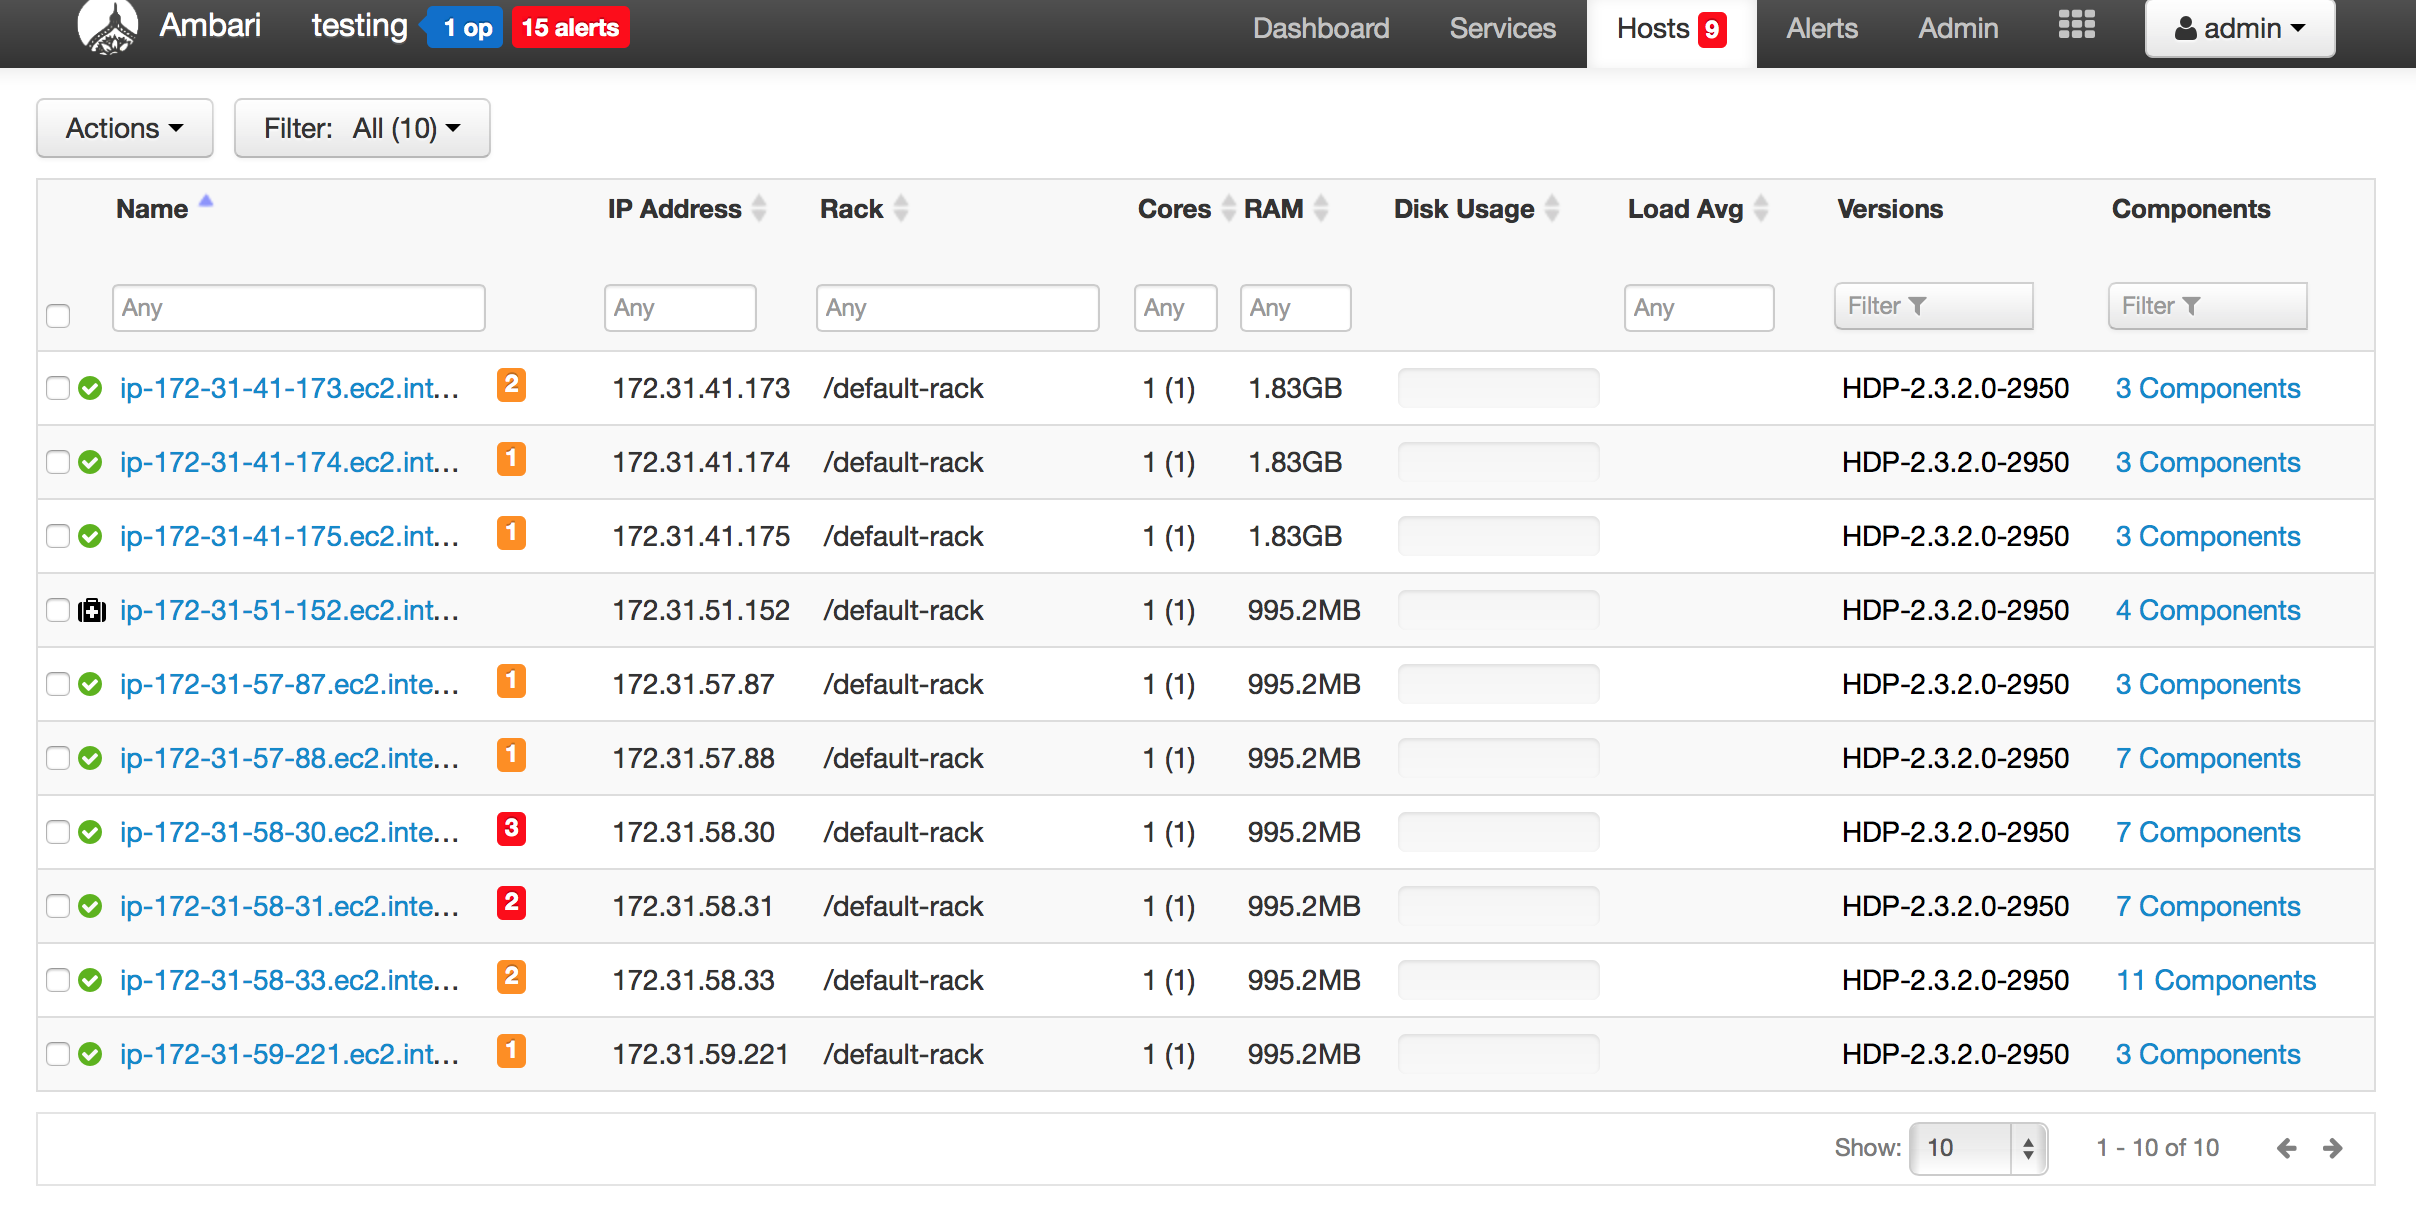
\includegraphics[width=0.7\textwidth,natwidth=1200,natheight=400]{deployment.png}
 \caption{Deployment Result}
 \end{figure}

\subsection{Deployment Problem}
During our deployment process, we encountered a problem that our Ambari Server cannot communicate with Ambari Agents. Thus, the server cannot execute the Hadoop cluster deployment commands.
\subsection{Solution to Deployment problem}
In order to figure out this problem, we analyzed the both log files of Ambari Server and Agents, and found that our Ambari Server cannot identify the hostname of Ambari Agents. For this problem, we tried two solutions.

The first solution is to register each agent��s IP address and hostname to Agent Server. The advantage is that it can help Ambari Server communicate with Agents. But the disadvantages of this solution are obvious, 1) The register process is complex. Since all agents need register to Ambari Server, and Ambari Server need execute shell scripts and add Agent's�� IP address and hostname into Server. 2) If Ambari Server is gone, the whole system will crush. When setting up a new Ambari Server, all agents need register again.

The second solution is to set up a DNS server for all Ambari Server and Agents. Here we adopt Consul to provide DNS server, which is a tool for discovering and configuring services in your infrastructure. The advantages of this solution are, 1) All Ambari Server and Agents need register to Consul once. 2) If a new Ambari Server is setup, it just needs get all Agents�� information from Consul. 3) It can increase the system��s robusticity and availability.

After comparing above two solutions, we adopted the second one to solve the problem, and this method can implement our solution pretty well.




\section{Monitor Hadoop YARN Cluster}
In order to scale the Hadoop YARN cluster, we should first decide whether it is necessary to scale out a cluster.  However, without monitoring data, the scale is misleading. Therefore, the first step we should take is to get the runtime information of the Hadoop eco-system.  \textbf{Figure 3} is the infrastructure that we have utilized to achieve monitoring module which served as the key decision for scaling feature.

\begin{figure}[h!]
 \centering
  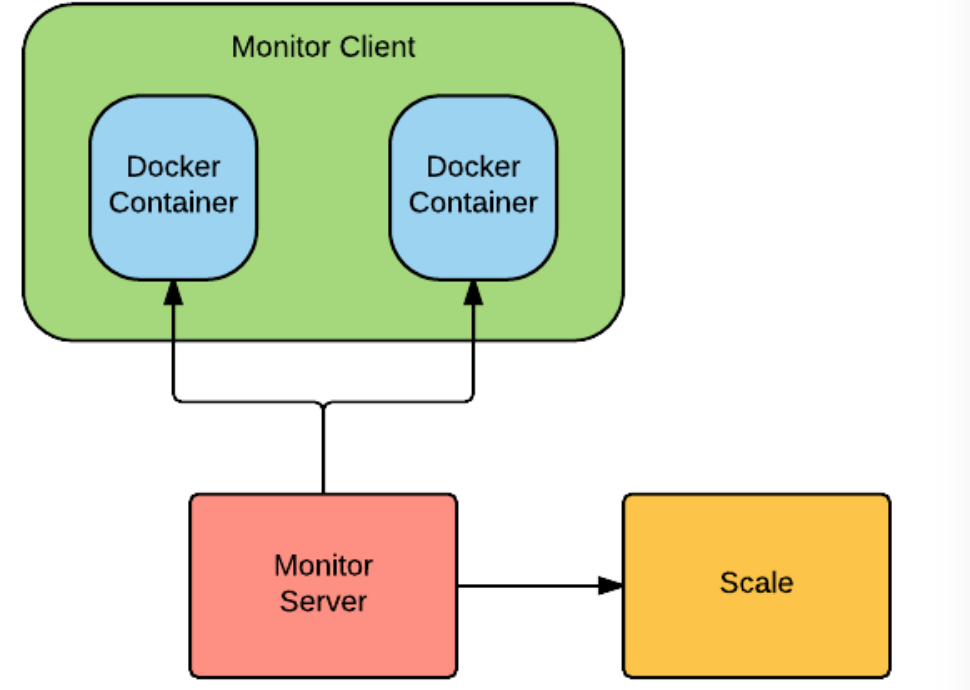
\includegraphics[width=0.6\textwidth,natwidth=500,natheight=300]{fig2.png}
 \caption{ Monitor Structure}
 \end{figure}

There are several ways that we can implement the infrastructure, such as through the Ambari Dashboard, the Amazon EC2 Monitoring Dashboard and implementing our own monitoring infrastructure such as Elasticsearch, Logstash and Kibana. We will then look into the data we get from Ambari Monitor Dashboard and EC2 metrics and decide whether we need more information in order to build a more applicable scaling strategy model for scaling cluster to improve the performance of MapReduce2 Job.
\subsection{Ambari Dashboard}
From Ambari Dashboard, we can get most information of the Hadoop system, HDFS status along with many Hadoop services such as ZooKeeper. We can add more widgets to the main dashboard to log more information and get the data from the widgets UI. We have run a sample Hadoop Job to get more understanding of how the monitoring data will look like.
\subsubsection{HDFS Monitoring Metrics}
For HDFS, the metrics are able to provide with the following data, shown in \textbf{table 1}. We can easily tell from the metrics that how much percentage disk is utilized by the DFS or System, which will contribute to the build of the scaling strategy model.
\begin{table}[h!]
\begin{center}
\begin{tabular}{ |c|c|c| }
\hline
NameNode & Started \\
\hline
SnameNode & Started \\
\hline
DataNodes & 1/1 Started \\
\hline
DataNodes Status & 1 live / 0 dead / 0 decommissioning \\
\hline
NameNode Uptime & 1.01 hours\\
\hline
NameNode Heap & 203.1 MB / 998.4 MB (20.3\% used)\\
\hline
Disk Usage (DFS Used) & 1.4 MB / 6.7 GB (0.02\%)\\
\hline
Disk Usage (Non DFS Used) & 4.9 GB / 6.7 GB (71.99\%)\\
\hline
Disk Usage (Remaining) & 1.9 GB / 6.7 GB (27.99\%)\\
\hline
Blocks(total) & 24\\
\hline
Block Errors & 0 corrupt / 0 missing / 24 under replicated\\
\hline
Total Files + Directories & 56 \\
\hline
Upgrade Status & No pending upgrade\\
\hline
Safe Mode Status & Not in safe mode\\
\hline


\end{tabular}
\end{center}
\caption{HDFS Monitor Metrics}
\label{table:1}
\end{table}

\subsubsection{YARN Monitor Metrics}
For YARN Monitor, we are able to get the following data as the \textbf{table 2} shows. We will have the Resource Manager Heap size and how many applications are currently submitted which are pending or running. The cluster memory information will also give us a hint whether to perform a scale.
\begin{table}[h!]
\begin{center}
\begin{tabular}{ |c|c|c| }
\hline
ResourceManager Heap & 16.8MB/989.9MB(1.7\% used) \\
\hline
Containers & 0 allocated/0 pending/0 reserved \\
\hline
Applications & {3 submitted/0 running/0 pending/3 completed/0 killed/0 failed}\\
\hline
Cluster Memory & {0 Bytes used/0 Bytes reserved/512.0 MB available}\\
\hline
\end{tabular}
\end{center}
\caption{YARN Monitor Metrics}
\label{table:1}
\end{table}

 Other than that, it also has the ability to monitor the CPU utilization of the instance as well as memory utilization and uptime information. \textbf{Figure 4} gives a brief snapshot of all the monitor data that we can get from the Ambari side.
\begin{figure}[h!]
 \centering
  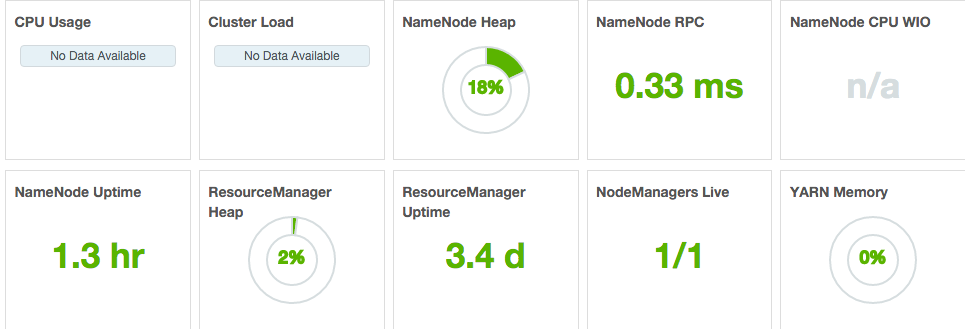
\includegraphics[width=0.8\textwidth,natwidth=1000,natheight=400]{fig4_2.png}
 \caption{Ambari Dashboard}
 \end{figure}
 \subsection{Amazon EC2 Dashboard}
 Other than Ambari Dashboard, which will give us more information about the Hadoop ecosystem. The monitoring metrics on EC2 will only provide with basic information on Instance level. It knows nothing about what is running on the instance. \textbf{Figure 5} gives us an illusion about the Monitoring metrics on Amazon. As we can see, the data is much less than Ambari provide us. However, the instance level information may also be useful to us, such as the network in/out, as it will give a hint about the network flow of the job which will help us to understand better how Data Intensive Computing works and know if the bandwidth of the network has something to do with our job performance.
\begin{figure}[h!]
 \centering
  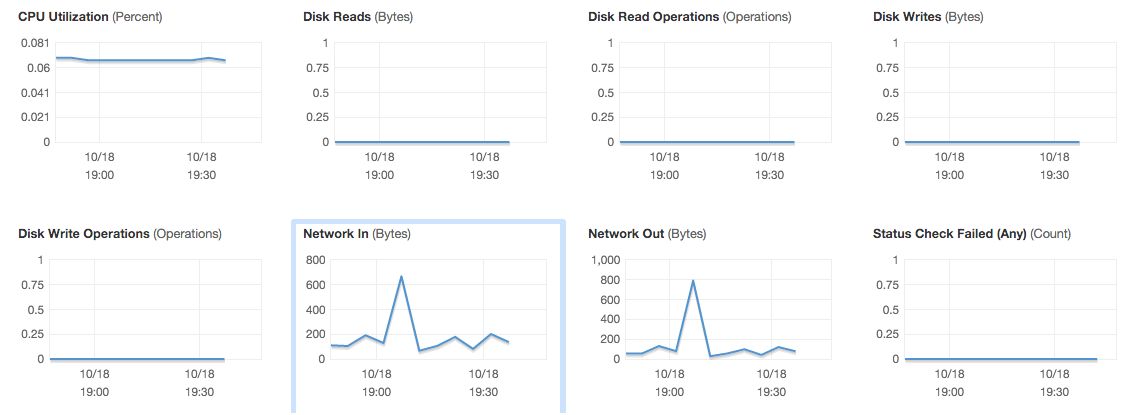
\includegraphics[width=0.8\textwidth,natwidth=1100,natheight=400]{fig4_3.png}
 \caption{Amazon EC2 Dashboard}
 \end{figure}

 \subsection{ELK}
 Elasticsearch, logstash combined with Kibana as a monitoring infrastructure is utilized by industry in recent years. No only we can get lots of logs from the system, we can also use it to monitoring our cluster to get some customized information which has not been provided by either Ambari or Amazon EC2. Since we are still not sure what kind of monitoring data will be used to build a scale strategy, no logs has been configured in the system to forward to ELK system. However, we think it is better to get started with the infrastructure in case we may need it later. \textbf{Figure 6} shows how data in Kibana Dashboard is visualized and \textbf{Figure 7} gives all the alternatives for data manipulation in Kibana can be achieved and visualized.
\begin{figure}[h!]
 \centering
  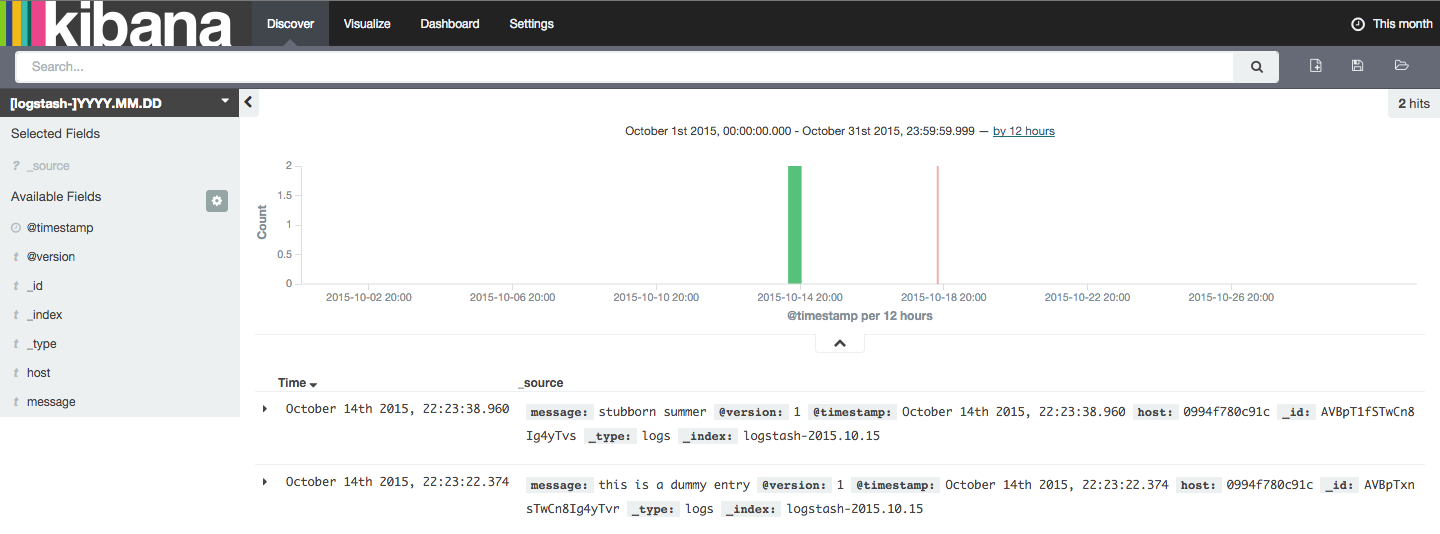
\includegraphics[width=0.9\textwidth,natwidth=1400,natheight=600]{fig4_4.png}
 \caption{Kibana Dashboard}
 \end{figure}

\begin{figure}[h!]
 \centering
  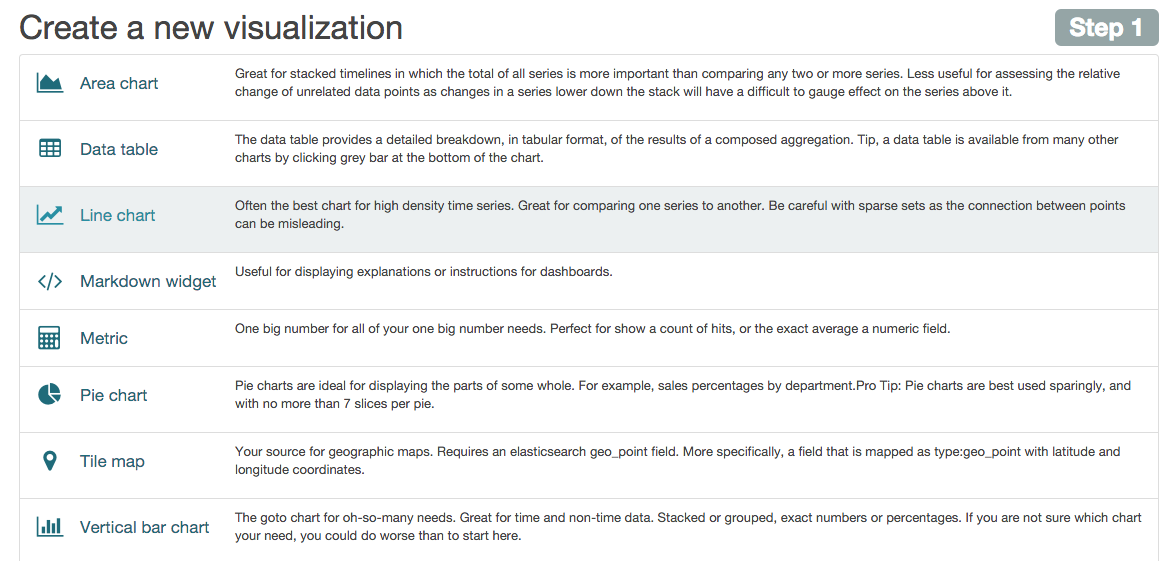
\includegraphics[width=0.9\textwidth,natwidth=1200,natheight=400]{fig4_5.png}
 \caption{Kibana function}
 \end{figure}
 \subsection{Conclusion}
 We believe the above three kinds of monitoring process will provide with sufficient data to build our scaling model according to different kinds of datasets and jobs. Therefore, less efforts will be spent on this section, we will be focusing more on scale part such as figuring the data set which can be used and how to make the scale actually works.


\section{Scale out Hadoop YARN Cluster}
For scaling out the YARN cluster, we divide this problem into three important sub problems.

The first problem is why we need to scale out. We expect scaling out could improve the performance. But some MapReduce jobs only process relatively small input data sets(several GBs), sometimes they are not suitable for scaling out. For other certain MapReduce jobs, we will figure out why these jobs need scale out the cluster based on our following experiments. Since AWS charges for the usage of EC2, we should control the cluster at a reasonable size for the tradeoff between cost and performance. We need to find a method to calculate the cost and design experiment to test performance.

The second problem is when we should scale out the cluster. For this problem, we should add slave nodes in the cluster as the dataset becomes larger,  and figure out how many slave nodes we should need adjust. In order to solve this problem, we will run different data sets and monitor the Hadoop Cluster, AWS EC2 performance and other related information. Then, based on these information, we will create our data model and give the results of when to deploy and how many data nodes should be adjusted.

The thirde problem is how we scale out the Hadoop Cluster. For this part, our current solution is to develop a scale-out server listening to the running cluster. When an adjustment event was fired, the server should be able to respond by add new hosts to the cluster or remove old hosts from the cluster.


\subsection{Experiment Design}
 The basic assumption here is that data intensive jobs are suitable for scaling out. The second assumption is that scaling out is necessary when the job exceeds a certain threshold of  YARN memory usage. These two assumptions are made from experience. So we will do experiments on different jobs and use result metrics to validate our assumptions. Our choices about experiment jobs, metris and clusters are described as following.\\
\textbf{Jobs}: Computing intensive jobs(like Pi estimate example) versus data intensive jobs(like word count example, tera sort example, log processing example)\\
\textbf{Metrics}: performance, performance per node,  performance per dollar: derive performance per dollar by dividing raw performance by the capital/acquisition cost of the hardware, cpu usage, YARN memory usage, I/O operation, network overhead. The metrics are already described  monitoring subsection.\\
\textbf{Clusters}: The initial cluster starts from 6 nodes. Each instance type is t2.micro equipped with 1G RAM and single CPU. Then scale out to 9 ,12 nodes of the cluster. (We are also  looking forward to get AWS credits to try scale-up instance which has larger RAM and multi-CPU)

Firstly, we did the experiment of Pi estimate example on cluster of 6 and 9 nodes, the cpu and memory usage is shown in \textbf{figure 8}. We found that the cpu and memory usage is small. And it is not a good test case to scale out. In the next step, we will do experiments on more example jobs and compare more metrics.
\begin{figure}[h!]
 \centering
  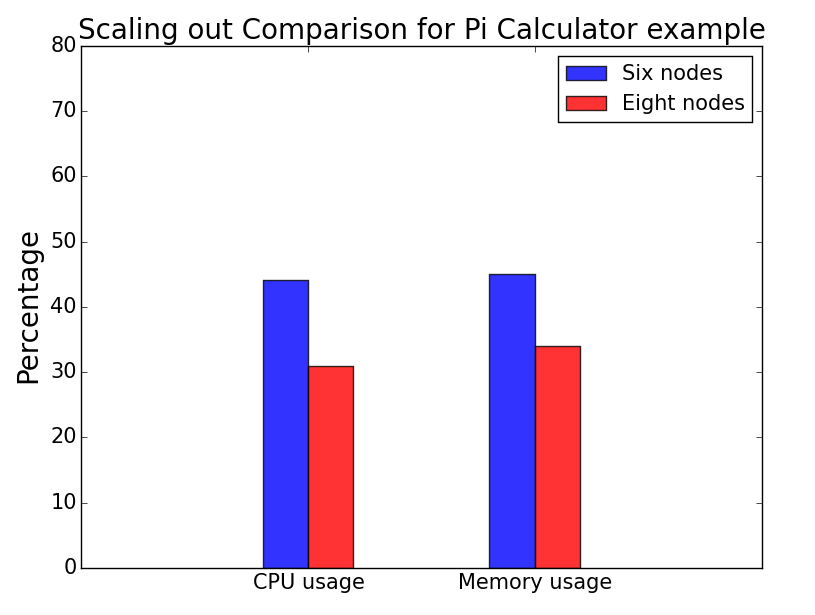
\includegraphics[width=0.4\textwidth,natwidth=500,natheight=400]{figureScale.png}
 \caption{Scaling System Workflow}
 \end{figure}

\subsection{ Auto Scale out Hadoop YARN Cluster}
We consider the cluster used in above experiment is static because the hardware resources are already given when the job is running. We manually modify the cluster size to compare the performance of running jobs. It leads to a question naturally about how to make the cluster itself decide add or remove on the fly. Thus the cluster��s throughput can be increased or decreased based on the cluster load and scheduled applications to achieve better performance without stopping the cluster.	

The key point here is to solve when to make an adjustment. Since we observed that the performance did vary when cluster size changed, the cluster adjustment should based on the real-time performance metrics. These metrics could be collected and queried by via elasticsearch. The YARN allocate resource based on memory, a simple schema is to ensure a stable memory usage of the cluster. This means when a memory usage exceed a maximum value, the cluster choose to add node or to remove when a low memory usage. The schema might make little difference to a single running job, but it is meaningful when multiple jobs submitted to the cluster. The process includes complicated balance of both hdfs data and YARN resource when cluster changed. We are still actively working on it. If the stable memory policy works, we can also apply similar policy like stable performance or stable cost to the auto-scale schema.

 \begin{figure}[h!]
 \centering
  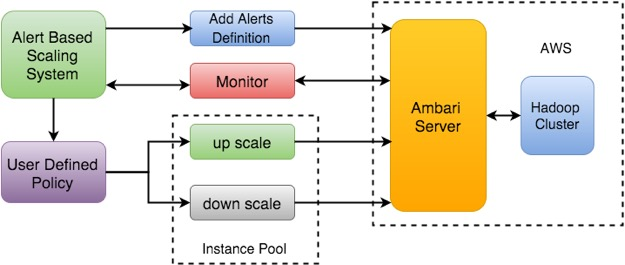
\includegraphics[width=0.8\textwidth,natwidth=1000,natheight=800]{scaling2.png}
 \caption{Scaling Process}
 \end{figure}
 
\begin{figure}[h!]
 \centering
  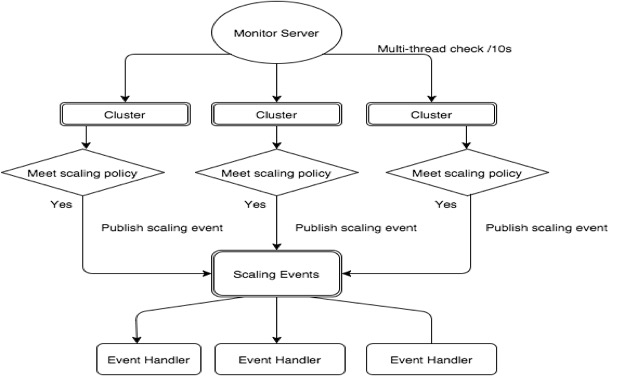
\includegraphics[width=0.8\textwidth,natwidth=1000,natheight=800]{scaling1.png}
 \caption{Scaling System Workflow}
 \end{figure}
 

 
\subsection{Case studies}
In the last, we run hadoop pi example to testify our auto scaling implementation.. The initial state of our cluster is one name node and three data nodes.  The scaling out demo  is to calculate pi based on quasi-Monte Carlo method. The number of maps is set to be 100. And the number of points to be generated is set to  ten million. If we set the alert to be 60\% of memory usage. And the usage of Yarn memory will reach 85\% after several minutes. And it will trigger the alert,  Our system gets the alert and executes the scaling out policy, that means adding 2 data nodes in this case. In practice, you can set both the alert and policy, like defining how long it takes to trigger the alert.
 \begin{figure}[h!]
 \centering
  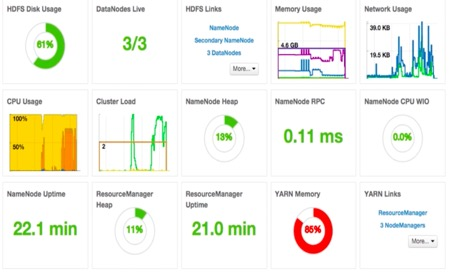
\includegraphics[width=0.8\textwidth,natwidth=1000,natheight=800]{scaling3.png}
 \caption{Scaling Out case}
 \end{figure}
 The scaling down demo is to remove data nodes from the cluster when there is no pending jobs.
\begin{figure}[h!]
 \centering
  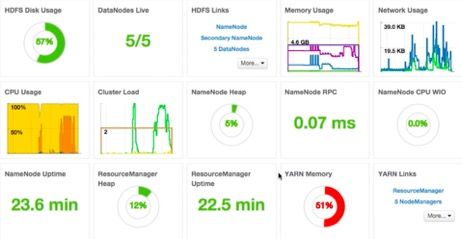
\includegraphics[width=0.8\textwidth,natwidth=1000,natheight=800]{scaling4.png}
 \caption{Scaling Down Case}
 \end{figure}
\section{Related Work}
In deployment, we used Go programming language library for aws and consul, a tool for discovering and configuring services in our infrastructure. In monitoring, our application integrates Hadoop provisioning and monitoring capabilities with the Ambari(an open-source, cluster-management tool ) and ELK stack(combine three open source projects Elasticsearch, Logstash, and Kibana). For scaling, although Hadoop cluster is widely used nowadays, many researchers[3,4] challenge the viewpoint that scaling out using a cluster of commodity machines is better to run data analytics workloads. Rowstron[3] argues that single big memory servers may simply be more efficient than clusters, which can substantially change price points and complexity.  Appuswamy[4] evaluates scaling up versus scaling out across a range of analytic workloads and using four metrics: performance, cost, energy, and server density. In the last part of our project, we want to do similar studies in scaling out. It is interesting and useful to conduct research in determining when and how to scale out the cluster.


\section{Conclusion}
During the deployment process, we have learnt a lot about how docker simplifies the process. Docker is lightweight and portable. Once we built the basic image of Hadoop, we can run it in each node without extra configuration. And during the configuration of the Elasticsearch, Logstash and Kibana, we have learned some basic knowledge about how the monitor and logging infrastructure works. Furthermore,  combining logstash forwarder and Ambari logs will give us the opportunity to generate statically real-time logs for us to analyse and work out a more efficient scaling model. For scaling, we made first step in running experiments to testify when and how to scale out the YARN cluster. In the future, there are two improvements for our experiments. One is to run different kinds of test jobs in Hadoop cluster. The other is to analyze the relationship between scaling out and various metrics like memory usage.


% Generate the bibliography.
\begin{thebibliography}{4}


\bibitem{Wadkar}
Wadkar, Sameer, and Madhu Siddalingaiah
\newblock Monitoring Hadoop.
\newblock  Pro Apache Hadoop. Apress, 2014. 203-215.

\bibitem{EC2}
http://docs.aws.amazon.com/AWSEC2/latest/CommandLineReference/ec2-cli-launch-instance.html

\bibitem{Rowstron}
Rowstron, Antony, et al.
\newblock Nobody ever got fired for using Hadoop on a cluster.
\newblock  Proceedings of the 1st International Workshop on Hot Topics in Cloud Data Processing. ACM, 2012.

\bibitem{Appuswamy}
Appuswamy, Raja, et al.
\newblock Scale-up vs Scale-out for Hadoop: Time to rethink?
\newblock Proceedings of the 4th annual Symposium on Cloud Computing. ACM, 2013.


\end{thebibliography}


\end{document}
